\section{Design of thread program model}
%这一部分,首先,我们将详细分析Phoenix较差scalability的根本原因,然后针对Phoenix scalability存在的challenge,我们提出可行的解决方案,即构造一种具有较好scalability的thread model。然后详细解释这种新的线程模型的详细设计方案,最后具体的实验部分在section 6
In this section, we first investigate the main factor of Phoenix's limited scalability, 
and then present a new thread model (\myth), which can achieve good scalability.
Finally, the detail design and implementation of \myth is given.


\subsection{Scalability of Phoenix}
%描述Phoenix 的 pool scalability
Phoenix uses shared-memory multiple threads to implement parallelism,
and programs written in Phoenix will start as many threads as the system’s cores.
\redt{Ideally, adding more threads and cores to the	runtime 
	would bring about a linear decrease in execution
	time.}
%However, the parallel scalability of Phoenix is not ideal.
However, Phoenix did not scale as well as expected.
As indicated by figure \ref{fig:phoenix:speedup}, 
when the system exceeds their scalability limitation, 
adding more cores might scale negatively.
That means the time of completing a workload increases if there are more cores in the system. 
% In general, the parallel scalability of Phoenix is poor.

%使用perf来收集热点函数的执行时间,实验结果显示,在32核情况下,(这里可以给出一个图,16和32核下的热点函数分别是什么,占用多少的百分比分别又是多少?)
%为了深入探究较差scalability的根本原因,
%我们利用Linux perf工具来收集程序的热点函数信息(主要看热点函数占用总运行时间的百分比),
%通过热点函数的分析,查看高核情况下,占用时间最多的运行函数,
%如表\ref{}显示,在16和32核情况下,各个应用程序中占用时间最多的函数。
%从表中可以看出,对一hist, lr, wc, sw,在32核情况下ticket\_spin\_lock的开销非常大,
%针对ticket\_spin\_lock,我们测试各应用程序的占用情况,如图\ref{}所示,
%从图中可以看出,
%随着核数的增多,各应用程序中的ticket\_spin\_lock的占用的开销越来越大,
%特别地,在16核和32核情况下,
%histgram中ticket\_spin\_lock占用的开销最大,分别为71.25\%和40.15\%.
%这表明,16核以上,hist, lr, wc, sm的运行时间主要用于锁的竞争和等待,
%而没有做实际的计算。
%并且随着核数的增多,这种竞争越激烈,导致Phoenix的scalability较差。
%事实上,从前面对Phoenix的分析我们知道,
%Phoenix中采取了划分和barrier两种策略,以避免多个map和reduce对同一个matrix竞争,
%然而实验的结果却显示在8核以上,依然有很激烈的竞争。
%函数的调用图显示,ticket\_spin\_lock几乎全部是由pagefault引起的。
In order to analyze the limited scalability behavior, 
Perf\cite{} is exploited to collect execution time  percent information of hot function. 
\redt{We observe that map function is the hot function as in low number cores, 
while ticket\_spin\_lock become the hot function in large number cores.
%However, the structure data shared by multiple threads in Linux kernel can cause the lock contention, which will degrade the scalability of Phoenix.
}
%To alleviate the overhead of lock, Phoenix has took two strategies to avoid multiple threads contending the share area.
Figure \ref{fig:phoenix:spinlock} shows the execution time percent of 
ticket\_spin\_lock on each benchmark. 
We observe that the cost of spinlock increases quickly as the cores number cross a specific value(ie.8).
%And in 32 cores, the \_\_ticket\_spin\_lock needs largest execution time for hist, lr, wc, sw.
Specially, hist with 16 and 32 cores shows that \_\_ticket\_spin\_lock is one function, 
which has largest execution times of 40.15\%  and 71.25\%, respectively. 

\redt{ticket\_spin\_lock is a type of spinlock which is caused by lock contention in Linux kernel.
	In Linux 3.2 kernel, ticket\_spin\_lock is used to ....
	Linux kernel won't scale well on multicores system: 
	that applications will spend an increasing fraction of their time in the kernel as the number of cores increases.
	Experiment results demonstrate that Phoenix will suffer from serious lock contention
	when the cores number exceeds 8. 
	That means most of execution time will be used for waiting but not actual computation.
Call-graph information shows that \_\_ticket\_spin\_lock is caused by pagefault.
That means pagefaults won't scale well on large numbers of cores:	
}


\begin{figure}[!h!t]  
    \centering
    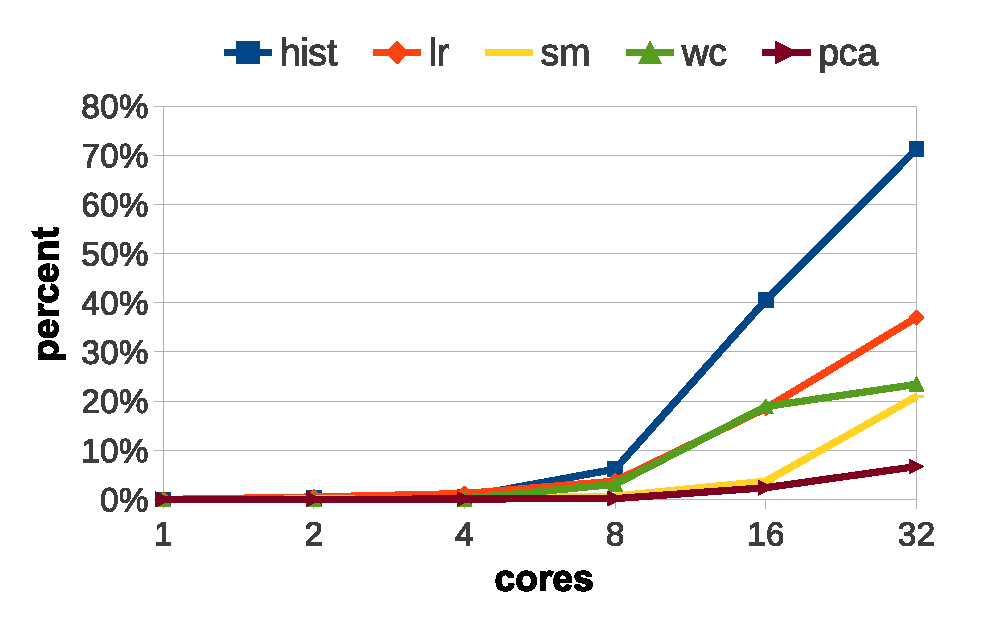
\includegraphics[width=0.35\textwidth]{eps/phoenix_spinlock.eps}
    \caption{Phoenix ticket\_spin\_lock percent}
    \label{fig:phoenix:spinlock}
\end{figure}


%Phoenix采取了划分和barrier的方式,以避免多个线程对共享区域的的竞争,为什么还会存在如此高的spinlock呢,
%\grayt{There is a sense in the community that traditional kernel
%designs won’t scale well on multicore processors: that
%applications will spend an increasing fraction of their time
%in the kernel as the number of cores increases.
%To understand the Linux scalability
%behavior, we analyze the related implementation of Linux
%kernel and exploit performance tools to identify scalability
%bottlenecks.
%}
%and source code analysis

%One reason that widely used operating systems 
%use a lock on the address space is 
%that they use complex index data structures to guarantee O(log n)
%lookup time when a process has many mapped memory
%regions. Linux uses a red-black tree for the regions\cite{linux}. 
%Because the data structures require rebalancing 
%when a memory region is inserted, 
%they protect the entire data structure with a single lock.
%The lock is local to a process address space.
%when the process is using multiple threads 
%then these threads will be able to access
%the address space in parallel, 
%which can cause contention on the lock.
%%随着核数的增多,这种问题会更加突出,最好导致较差的scalability
%\bluet{As the increasing of cores number, 
%	the scalability will be bad.
%}




The mmap() system call is utilized to read in input data. 
Once the user passes the pointer of the mmaped region to runtime as an argument, 
multiple map threads will concurrently cause pagefault in the input data when they invoke map functions.
All these pagefaults will contend the unique mmap\_sem semaphore
which is used for protecting the address space shared by multithread.
One reason that Linux uses a single semaphore on the address space is 
that it needs a red-black tree to guarantee O(log n)
lookup time when a process has many mapped memory regions\cite{linux}. 
%Since the red-black tree requires re-balance when a new memory region is inserted, 
%Linux protect the entire data structure with a single semaphore.
As the semaphore is local to a process address space,
%when the process is using multiple threads, 
%then these threads will be able to access the address space in parallel, 
concurrently accessing will cause contention on the semaphore
when the space is shared by multiple threads.
The semaphore is a sleep lock and may run into convoying problems,
where waiting threads may get stuck at the end of the wait queue for a long time.\cite{Andi2009lmulticore}
The contention is intense when there is a large  number of threads,
thus the parallel scalability of the benchmark will degrade.
%Therefore, when performing many threads,  the spinlock contention will degrade the parallel scalability performance of the benchmark.

%Data structure private locks can be a problem 
%if the data structure is shared by multiple threads. 
%A standard example here are the mm\_sem read-write semaphore 
%that protects the list of mappings in a process and 
%the pagetable\_lock that protects the pagetable state of a process. 
%These locks are local to a process’ address space. 
%\bluet{In Phoenix, there is one master process,
%and map worker or reduce worker are threads belong to the master process}. 
%However when the process is using multiple threads 
%then these threads will be able to access the address space in parallel,
%which can cause contention on these locks.
%Call-graph information
%and source code analysis show that the two functions are
%called when adding a virtual memory address range into the
%process address space or deleting a virtual memory address range. 




%Unfortunately these programs are often written to start as many threads as the system has CPUs, 
%but when the system is larger than their scalability limit adding more threads might actually scale negatively.
%The first measure is to limit them to the maximum number of threads that they can successfully scale to.
%This of course leaves some of the CPUs idle. 




%The difference between processes and threads under Linux 2.4 is that threads share more parts of their state (address space, file handles etc) than processes, 

\subsection{Scalable thread model}
%这一部分,我们不提生产消费模型,
%为什么要进行地址空间隔离,通过新的线程模型,我们实现了地址空间隔离,隔离之后有什么好处?相比Phoenix,我们这种新的模型会不会带来开销。

Our goal is to make pagefaults scale to large numbers of cores.
There are many way to achive this target such as \cite{Clements2012Scalable}\redt{...}.
%However, We don't want to change the implementation of operating system, but just provide a easy-to-use scalable thread model.
In fact, if applications use processes instead of threads can avoid a single shared address space, but this complicates sharing.
However, We don't want to change the implementation of operating system or employ process to program, but just provide a modified thread model with elevated scalability.
This requires addressing a basic problem, how allow pagefaults to eliminate on the per-process read/write semaphore, when multiple threads run concurrently.
At the same time, we aim at providing an easy-to-use programming abstraction to support scalable MapReduce.

To address the problem and achieve our goal, we propose a new thread programming model \myth(Scalable thread). 
%we persents a new concurrent address space design 
%that eliminates the above sources of contention by applying a new program model and by introducing channel, a way to share data between threads.
%We aim at providing an easy-to-use programming abstraction to support scalable MapReduce.
%With this target, we propose a new thread programming model \myth(Scalable thread).
%We propose a new thread programming model to support efficient pipeline parallelism.
%新的线程模型与传统的Pthread模型的主要不同在于:(1)每个线程拥有自己独立的地址空间,这样可以避免多个线程对mm\_struct结构的竞争。(2)线程之间有一个共享的通道,同于线程数据的共享。
\myth is C library-based.
On the one hand, threads in \myth run in separate memory spaces, eliminating the contention on the single semaphore. 
%Threads in Pthreads share the address space of the process that created it, 
%while threads in \myth have their own address space,
%meaning each thread has a mm\_struct.
%Therefore, thread no need contend with others thread for lock.
On the other hand, threads based on share space can directly communicate with other threads of its process; 
While \myth must use interprocess communication to communicate with the other threads.
We provoide a share channel for threads to communicate.


\label{sec:pm:thread}
\begin{figure}[htpb]
\input chanapi.tex
\caption{Main functions of \myds thread API.}
\label{fig:api:thread}
\end{figure}

%mapreduce中是如何使用这个简易的模型进行编程和实现的,这个模型潜在的开销是什么
Figure\ref{fig:api:thread} lists main function of managing threads and channels in \myth.
At initial stage of \myds, the master thread invoke \codet{thread\_alloc} to create map and reduce workers, 
and then creates and sets up channels for communication between each pair of map worker and reduce worker by invoking \codet{chan\_alloc}.
After that, the master starts all workers by invoking \codet{thread\_start}.
The master invoke \codet{chan\_setprod} to set a thread as a producer to send message to channel, and \codet{chan\_setcons} to set thread as a consumer to receive message from channel, respectively. 
which is a producer-consumer model.(We will describe it in Section 4). 

Though, using \myth can decrease the overhead of contention,
it also take some extra overhead comparing to Phoneix. 
The extra overhead focus on initialization(section 5). 


\subsection{Design of the Channel}
%channel的底层实现,以及它无限制的映射机制,想说明的问题是:不需要等待,且没有过多的malloc和free操作带来的开销。
Once the channel relationships are set up, 
map workers can invoke \codet{chan\_send} to send key-value to corresponded channel,
and the reduce workers can receive from the channel by \codet{chan\_recv}.
In order to avoid map waiting when the channel buffer is full,
we design an unbounded size of communication buffer for channel.
That means a sender can send any number of messages without blocking or waiting.
As a result, system can achieve high throughput.
%Unboundedness goal is the key to achieve high throughput.
%这个特性的好处


%无边界的channel的实现,依赖于底层的extend机制,
%它允许将channel buffer区域重新映射到一块新的物理地址,
%并且不影响consumer对旧的物理的读取。
%channel buffer对应producer和consumer地址空间中一块区域,
%我们称之为\codet{CHAN}区域,有一个pagetable(\codet{ptab})用于管理该区域的物理地址映射。
\begin{figure}[!h!t]  
	\centering
	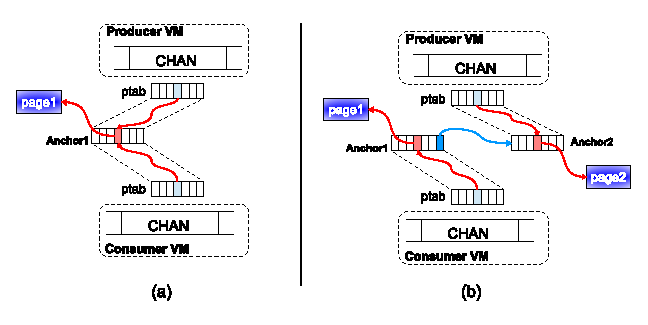
\includegraphics[width=0.5\textwidth]{eps/chan_extend.eps}
	\caption{channel extend machanism}
	\label{fig:spmckern:extend}
\end{figure}
In order to reach a unbounded buffer,
We design an extend mechanism 
which allows remap channel’s buffer to a new page frames,
and consumer can read the old page frames at the same time.
In our design, channel buffer is a virtual memory area \code{CHAN}
in the producer and consumer address space.
There is a pagetable(\code{ptab}) to store the mapping between virtual addresses and physical addresses, with each mapping as a corresponding page table entry(\code{PTE}).

%extension
Initially, the system will not allocate the actually page frames for \code{CHAN} area but a a special anchor page(\codet{Anchor1}),
which is shared between producer and consumer.
That is each entry(pte) in \code{ptab} points to the address of Anchor1.
When the producer need send message, 
writing the data to CHAN, a pagefault will take place.
Upon a producer page fault, the fault handler will allocate a real page frame(\code{page1}) and the \code{Anchor1}'s \code{pte} point to the page. 
Then producer can locate the page by \code{pte} and the data need to send will copy to this \code{page1} lastly.
After sending, consumer can locate the written page\code{page1} by pte 
and read it.

If the channel buffer(\code{CHAN}) area is full, 
producer no need to writing, 
but just remap \code{CHAN} to another anchor \code{Anchor2},
so that the producer can write the page afterwards.
To record and trace generations of page frames among old page frames 
and new page frames, a extension PTE is introduced.
That mean,
it can call extend primitive to remap channel buffer to new page frames,
without changing the old page that consumers may still require. 
Consumer can use the extension \code{pte} to locate the new
After a consumer receive the old page from the channel, 
it can call extend to find the new page frames sended by the
producer.
The older page frames decrease their reference counts and
are freed automatically when the counts reach zero.






 
%a special anchor extension page is introduced and shared between producer thread and consumers consumer.
%Initially a sequence of pages in channel buffer 
%are mapped to a \codet{anchor} page table (Anchor in Figure
%\ref{fig:spmckern:extend}), 
%in which each page has a corresponding page table entry (PTE).
%Upon a producer page fault, the fault handler will allocate a real page frame and update the faulting page with a
%writable producer mapping so that the producer can write the
%page afterwards.
%When a thread want to send without waiting, 
%it can call extend primitive to remap channel buffer to new page frames,
%without changing the old page 
%that consumers may still require. 






%\begin{figure*}[htpb]
%	\centering
%	\subfigure[when the channel buffer is not full]{
%		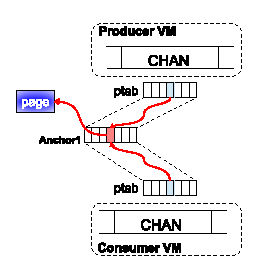
\includegraphics[width=0.35\textwidth]{eps/chan_extend1.eps}
%		\label{fig:dmr:chan:extend1}
%	}
%	\subfigure[the channel buffer is full, remapp the buffer to a new]{
%		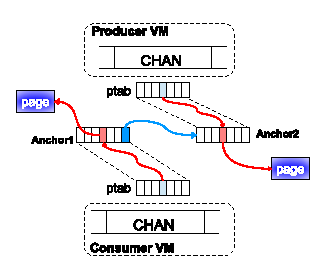
\includegraphics[width=0.45\textwidth]{eps/chan_extend2.eps}
%		\label{fig:dmr:chan:extend2}
%	}
%	\caption{Extend mechanism of channel in \myth}
%	\label{fig:time}
%\end{figure*}

In the follow section, we will describe \myds, 
which is based on \myth.
we focus on how the producer-consumer model and unbounded channel be used in \myds.








